\documentclass{beamer}

%%%%%%%%%%%%%Solarized Theme%%%%%%%%%%%%%%%
\usecolortheme[dark,accent=cyan]{solarized}
\beamertemplatenavigationsymbolsempty
%%%%%Packages%%%%%
\usefonttheme{serif}
\usepackage[T1]{fontenc}
\usepackage[utf8]{inputenc}
\usepackage[english]{babel}
\usepackage{fontawesome}
\usepackage{minted}
\usepackage{soul}
\usepackage{ulem}
\usepackage{blkarray}
\usepackage{multirow}
\usepackage{algorithm2e}
\usepackage{pgf}

\definecolor{DarkGray}{gray}{0.1}
\usemintedstyle{paraiso-dark}
\definecolor{Gray}{gray}{0.92}

\usepackage{graphicx}
\usepackage{hyperref}
\usepackage{colortbl, xcolor}
\usepackage{booktabs}
\usepackage{amsmath,amsthm, amssymb, latexsym}
\usepackage{multicol}
\usepackage{tikz}
\usepackage{xcolor}
\usepackage{graphicx,multirow}
\usetikzlibrary{calc, shapes, patterns}
\definecolor{plain}{rgb}{93,93,93}
\usetikzlibrary{positioning,arrows}
\definecolor{applegreen}{rgb}{0.55, 0.71, 0.0}
\usetikzlibrary{decorations.pathreplacing, backgrounds, fit}
\usetikzlibrary{graphs,graphs.standard}
\usetikzlibrary{calc,matrix}
\usetikzlibrary{trees,positioning,arrows,chains,shapes.geometric,%
    decorations.pathreplacing,decorations.pathmorphing,shapes,%
    matrix,shapes.symbols}

\tikzset{
>=stealth',
  punktchain/.style={
    rectangle, 
    rounded corners, 
    % fill=black!10,
    draw=solarizedBase3, very thick,
    text width=10em, 
    minimum height=3em, 
    text centered, 
    on chain
    },
    individual/.style={
        rectangle, 
        rounded corners, 
        % fill=black!10,
        very thick,
        text width=17em, 
        minimum height=3em, 
        text centered},
  tuborg/.style={decorate, thick, solarizedBase3},
}
\tikzstyle{cooperator} = [rectangle,
color=solarizedBlue!70, draw=solarizedBlue, text width=.25cm, outer sep = 2pt]
\tikzstyle{defector} = [rectangle,
color=solarizedRed!70, draw=solarizedRed, text width=.25cm, outer sep = 2pt]
\tikzstyle{score} = [rectangle,
color=solarizedOrange!70, draw=solarizedOrange, text width=.25cm, outer sep = 2pt]

\usepackage{standalone}
\usepackage{siunitx}

\begin{document}

\begin{frame}
    \begin{center}
        \Large{\textcolor{orange}{A computational approach to cooperation}} \\
        \vspace{.5cm}

        \vspace{1cm}
        \normalsize{Tuesday Lunch} \\
        \vspace{.5cm}

    \end{center}
\end{frame}


\begin{frame}
    \begin{center}
    
\includegraphics[width=0.24\textwidth]{static/mpi.jpg}\hspace{8pt}
    
\includegraphics[width=0.24\textwidth]{static/cardiff_uni_logo.png}\vspace{8pt}

    
\includegraphics[width=0.24\textwidth]{static/ssi-logo.png}\hspace{8pt}
    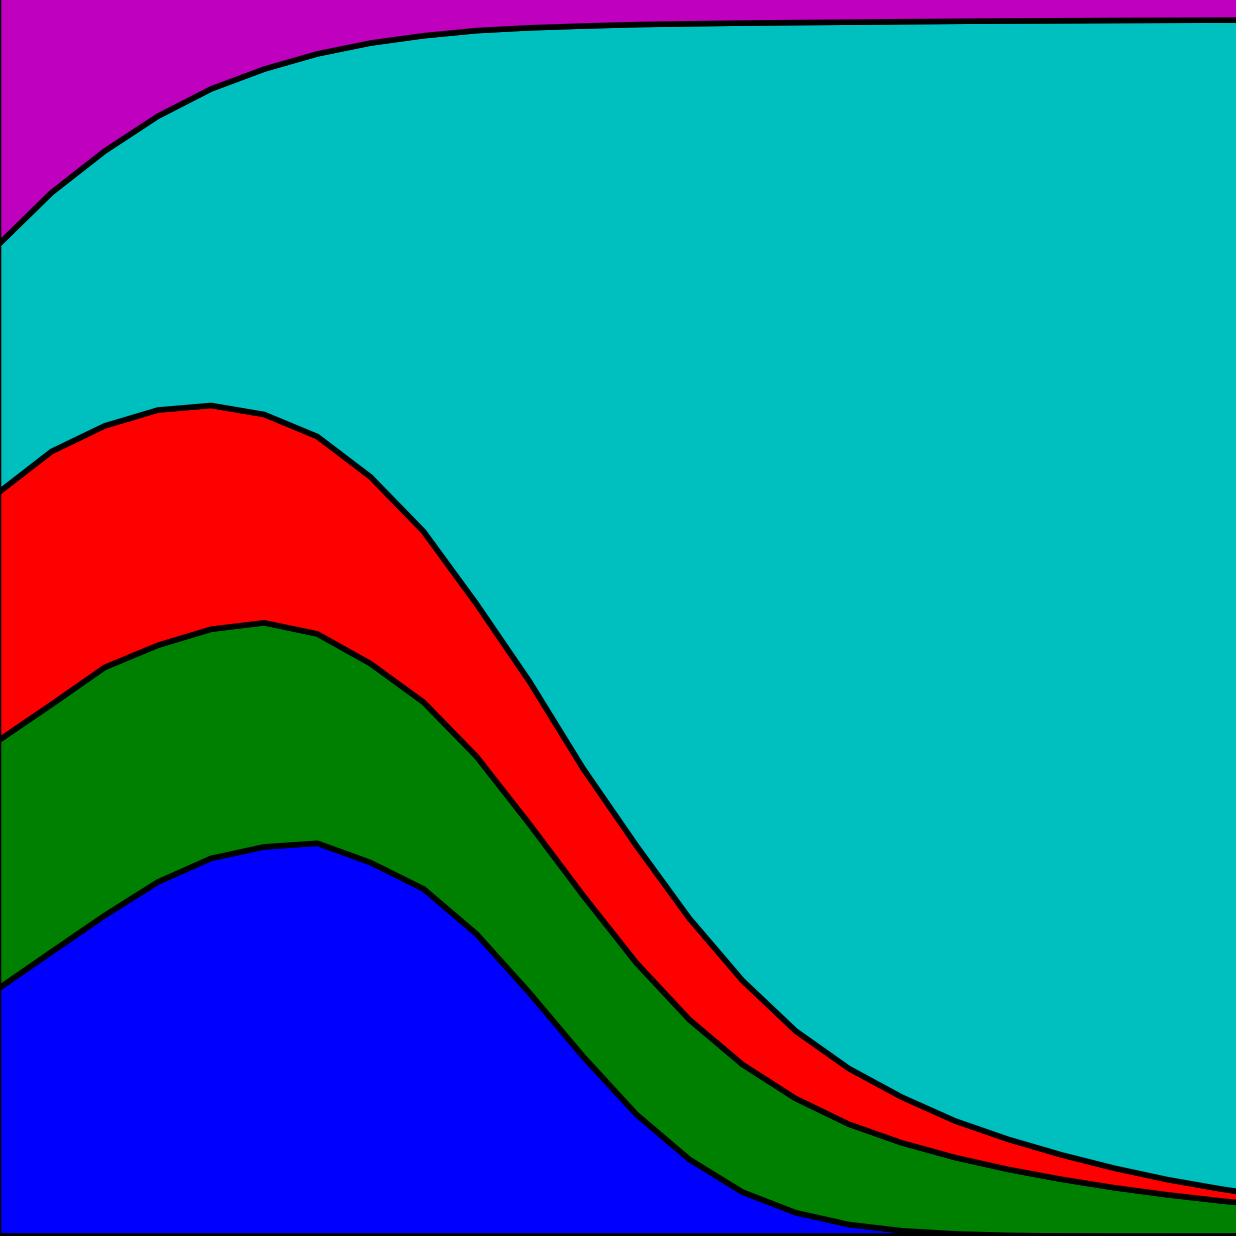
\includegraphics[width=0.24\textwidth]{static/axelrod-logo.png}
    \end{center}
\end{frame}

\begin{frame}
    \begin{center}
        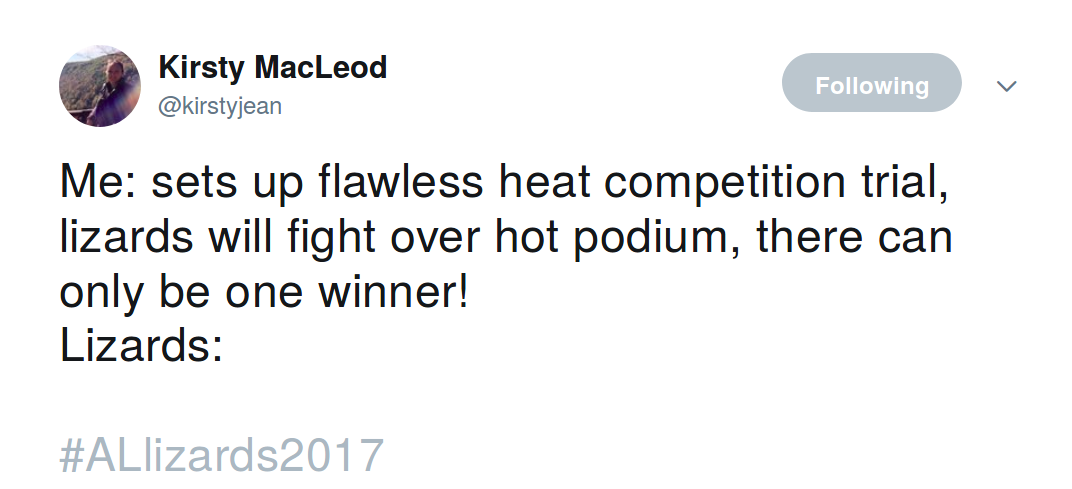
\includegraphics[width=.7\textwidth]{static/lizard-tweet.png}
    \end{center}
    \begin{center}
        \pause
        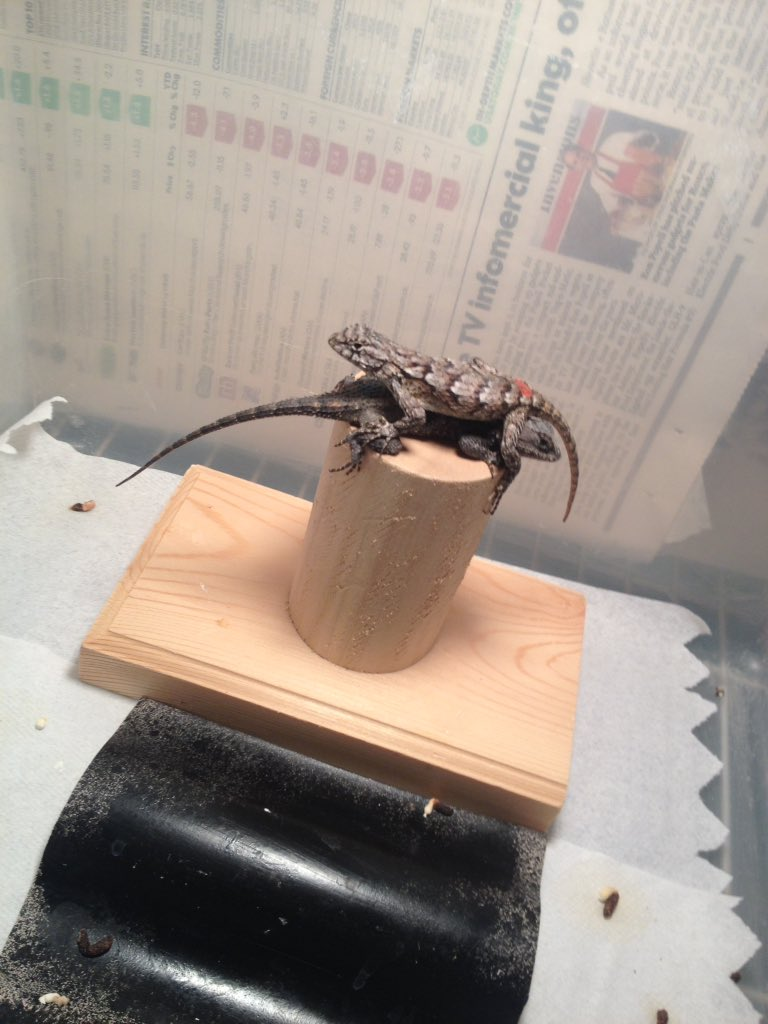
\includegraphics[width=.35\textwidth]{static/lizard-cooperation.jpg}
    \end{center}
\end{frame}

\begin{frame} \textbf{
    \begin{center}
    \Huge{
        \begin{equation*}
            \begin{blockarray}{c(cc)}
                 & (3, 3) & (0, 5) \\
                 & (5, 0) & (1, 1) \\
            \end{blockarray}
        \end{equation*}}
    \end{center}}
\end{frame}

\begin{frame}
    \begin{center}
    \includestandalone[width=\textwidth]{static/iterated_prisoners_dilemma}
    \end{center}
\end{frame}

\begin{frame}
    \begin{center}
    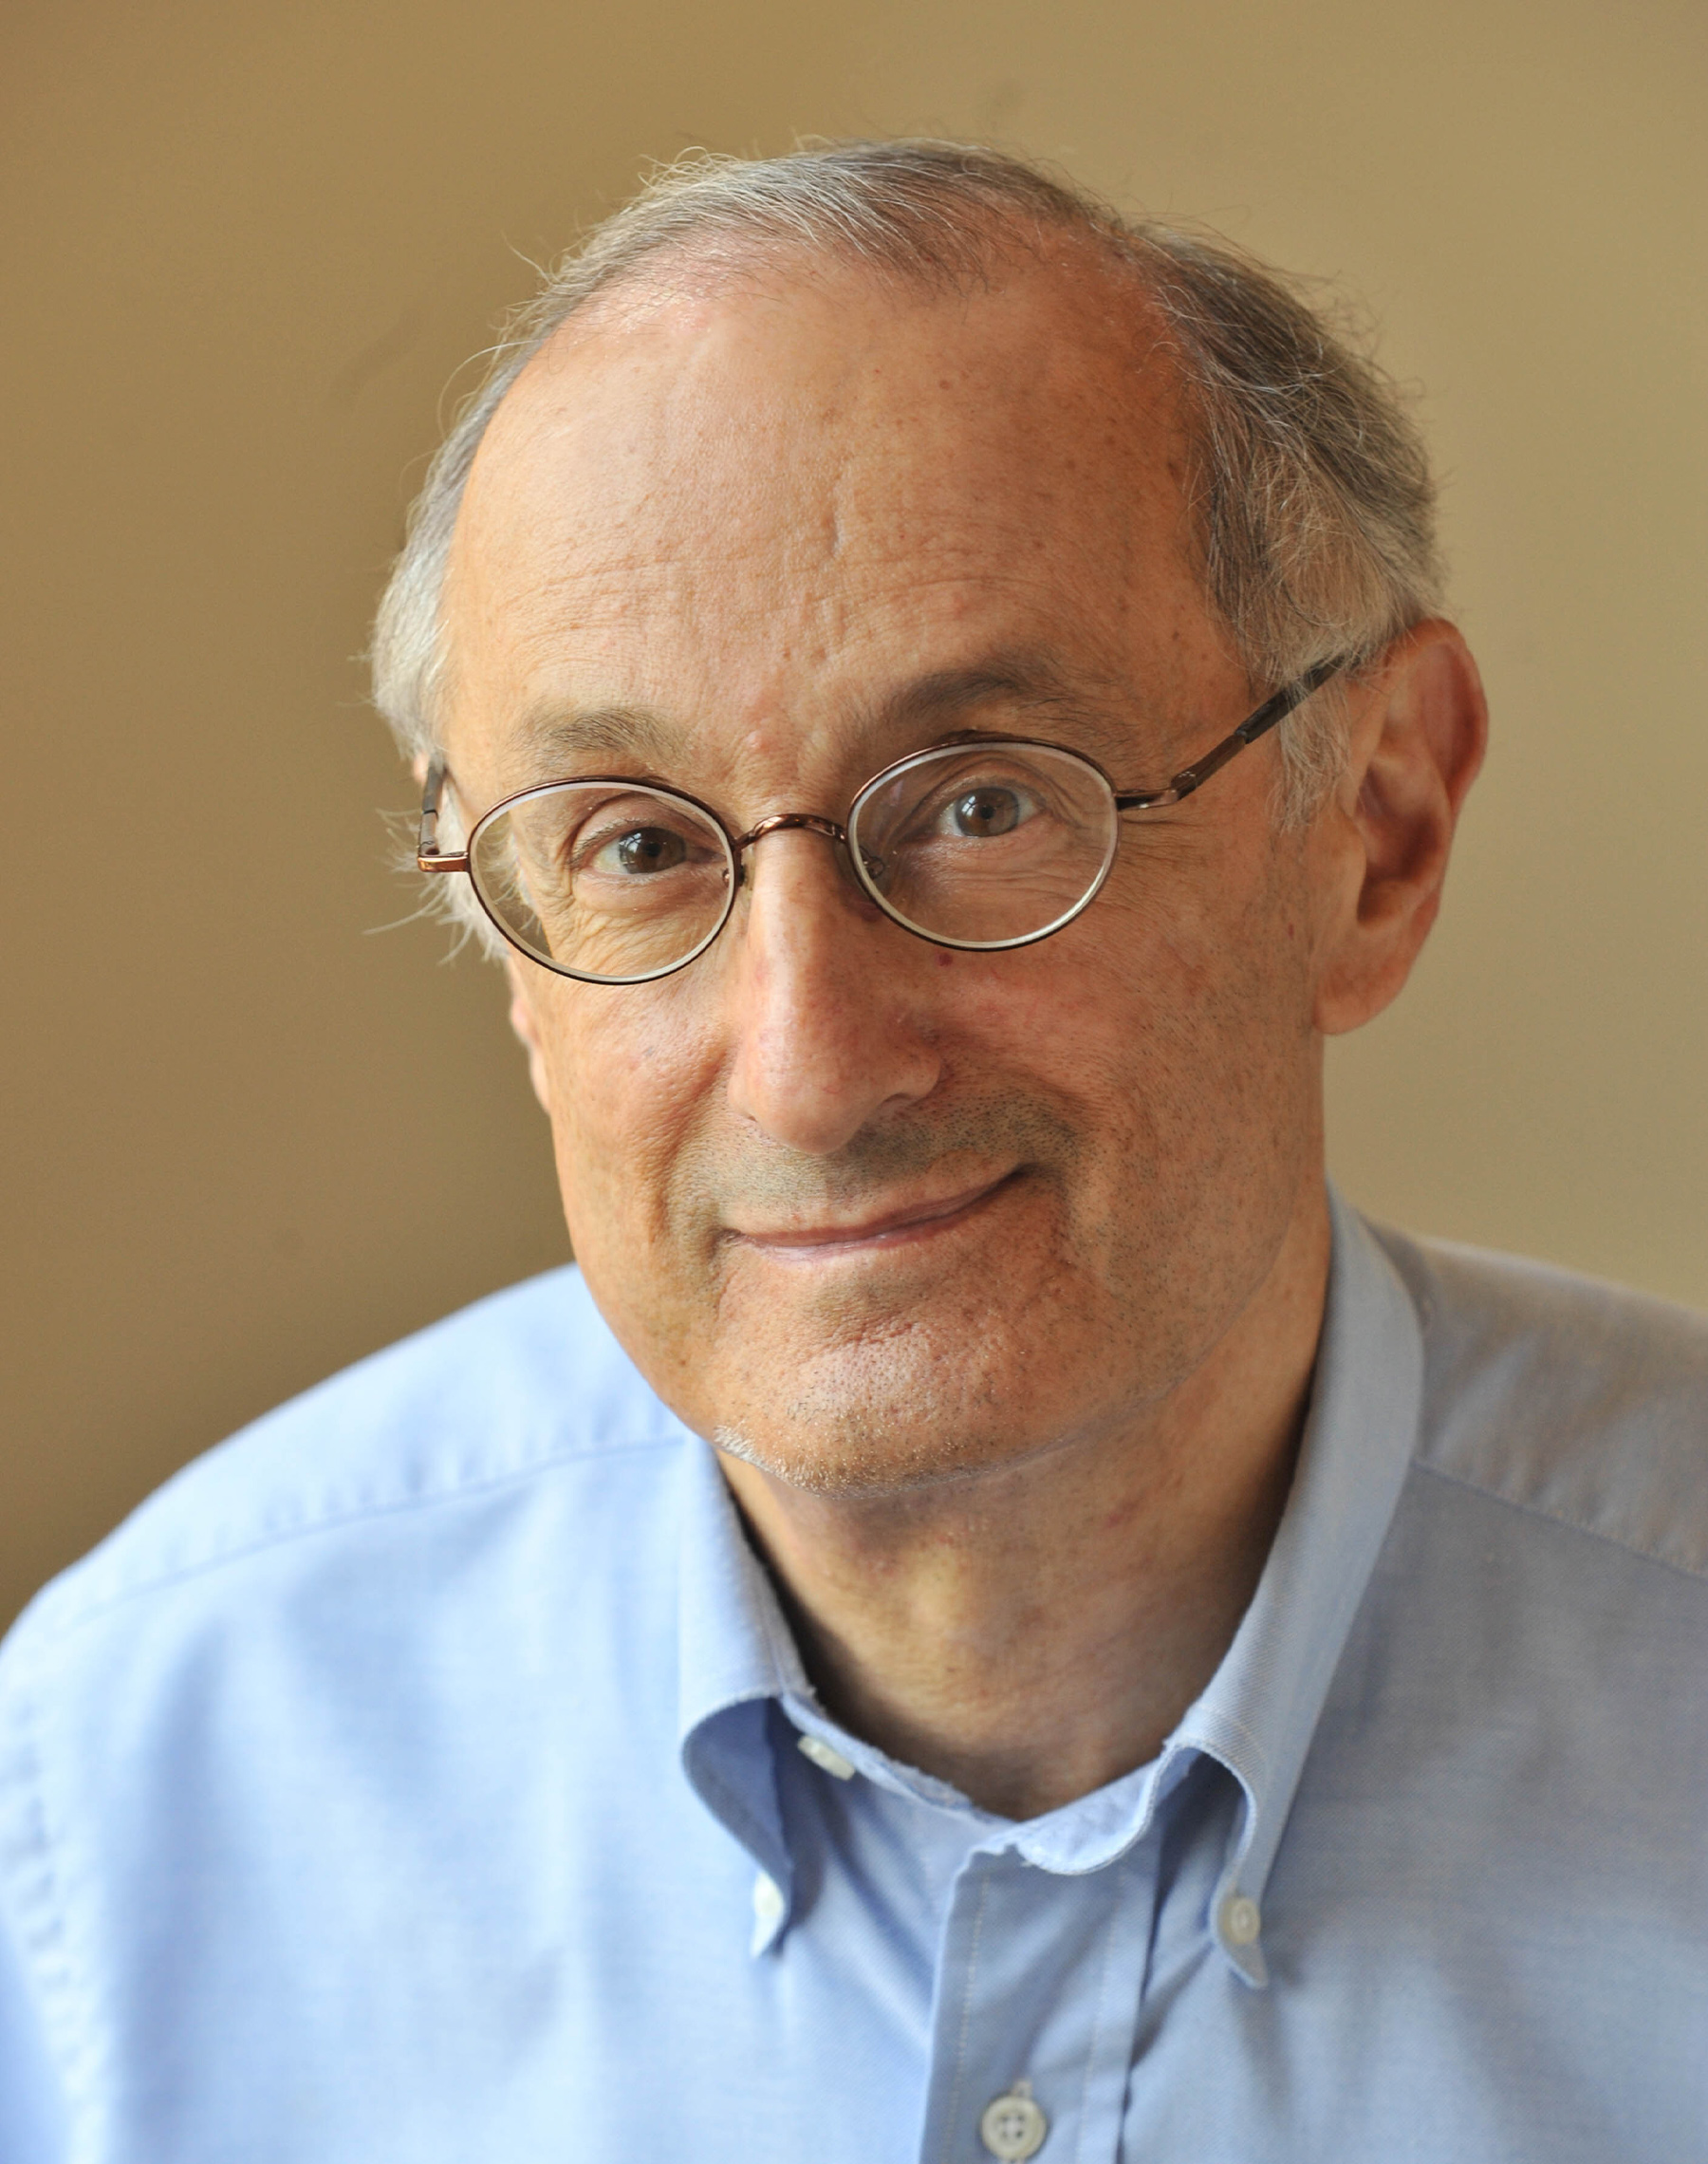
\includegraphics[width=.55\textwidth]{static/axelrod-robert.jpg}
    \end{center}
\end{frame}


\begin{frame}
    \begin{center}
    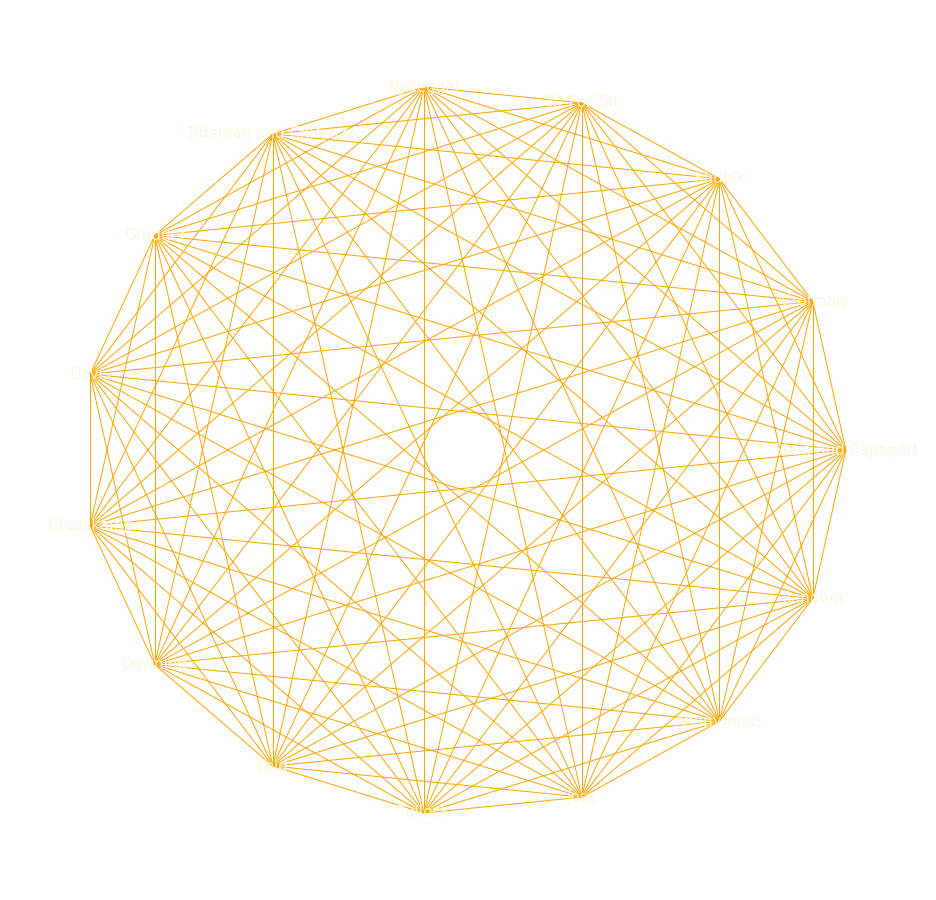
\includegraphics[width=.75\textwidth]{static/first_tournament}\\
    \vspace{1cm}

    \tiny{Effective Choice in the Prisoner's Dilemma. R. Axelrod. Journal of Conflict Resolution}
    \end{center}
\end{frame}

\begin{frame}
    \begin{center}
    
\includegraphics[width=.75\textwidth]{static/second_tournament}\\
    \vspace{1cm}

    \tiny{More Effective Choice in the Prisoner's Dilemma. R. Axelrod. Journal of Conflict Resolution}
    \end{center}
\end{frame}

\begin{frame}
    \begin{center}
        
\includegraphics[width=.09\textwidth]{static/crown.png} \\
        \Large{Tit For Tat} \\
        \vspace{1cm}

        \small{``A strategy that starts by cooperating and then mimics the previous action of the opponent."}
    \end{center}
\end{frame}

\begin{frame}
    \begin{enumerate}
        \item Be ``nice''; Do not be the first to defect
        \item Do not be envious; by striving for a payoff larger than the opponent's payoff
        \item Do not be too clever
        \item Reciprocate both cooperation and defection; Be provocable to retaliation and forgiveness
    \end{enumerate}
\end{frame}

\begin{frame}
    \begin{center}
    \includestandalone[width=.75\textwidth]{static/strategies}
    \end{center}
\end{frame}

\begin{frame}
    \begin{center}
    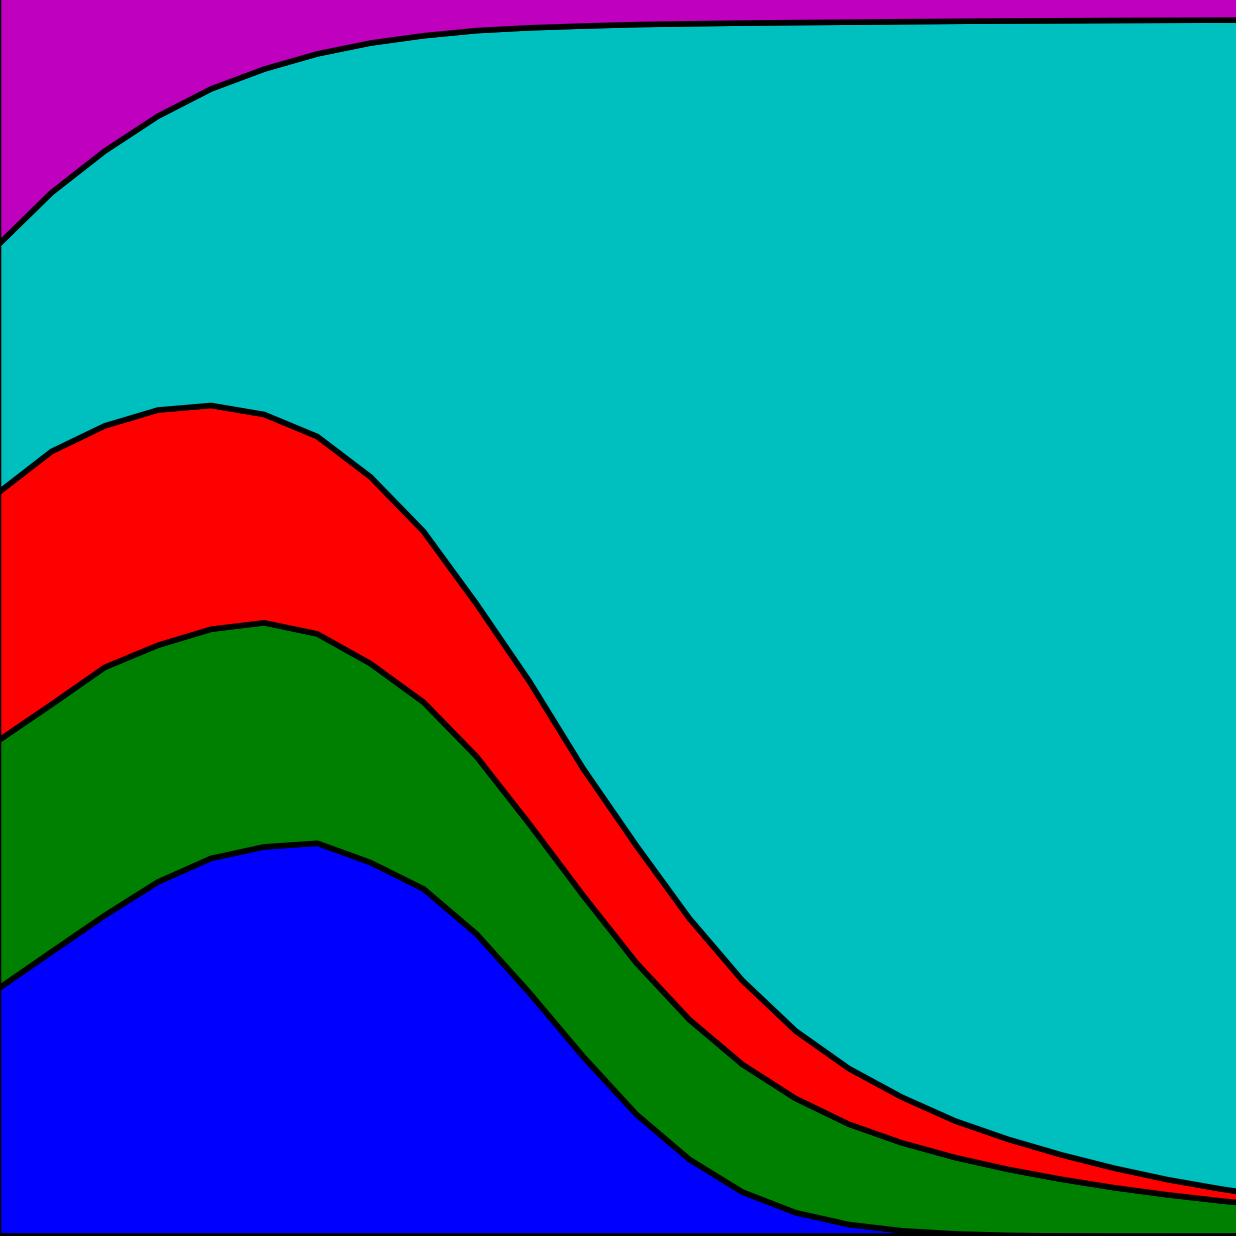
\includegraphics[width=.35\textwidth]{static/axelrod-logo.png} \\
    \vspace{1cm}

    \tiny{An open framework for the reproducible study of the Iterated prisoner's dilemma. Vincent Knight, Owen Campbell, Marc Harper et al. Journal of Open Research Software}

    \end{center}
\end{frame}

\begin{frame}
    \begin{center}
        \Large{150} \small{strategies from the literature} \\
        \vspace{1cm}
        \pause
        \Large{239} \small{strategies available today}
    \end{center}
\end{frame}

\begin{frame}[fragile]
	\begin{minted}
    [
    framesep=4mm,
    baselinestretch=1.2,
    bgcolor=DarkGray,
    fontsize=\tiny,
    ]
    {python}
    import axelrod as axl

    players = [axl.SuspiciousTitForTat(),
    ...        axl.HardTitForTat(),
    ...        axl.OmegaTFT(),
    ...        axl.Gradual(),
    ...        axl.WinStayLoseShift()]

    tournament = axl.Tournament(players,
    ...                         turns=200,
    ...                         repetitions=5)
    
    result = tournament.play()
    \end{minted}
\end{frame}


\begin{frame}
    \centering
    A meta analysis of tournaments and an evaluation of performance in the Iterated Prisoner's Dilemma. \\
    \vspace{.5cm}

    \tiny{Nikoleta E. Glynatsi, Vincent A. Knight, Marc Harper} \\
    \vspace{.5cm}

    \tiny{arxiv.org/abs/2001.05911} \\
    \vspace{.8cm}

    \tiny{Axelrod-Python v.3.0.0. - 195 strategies}
\end{frame}

\begin{frame}
    \begin{center}
    \includestandalone[width=\textwidth]{static/data}
    \end{center}
\end{frame}

\begin{frame}
        \begin{center}
        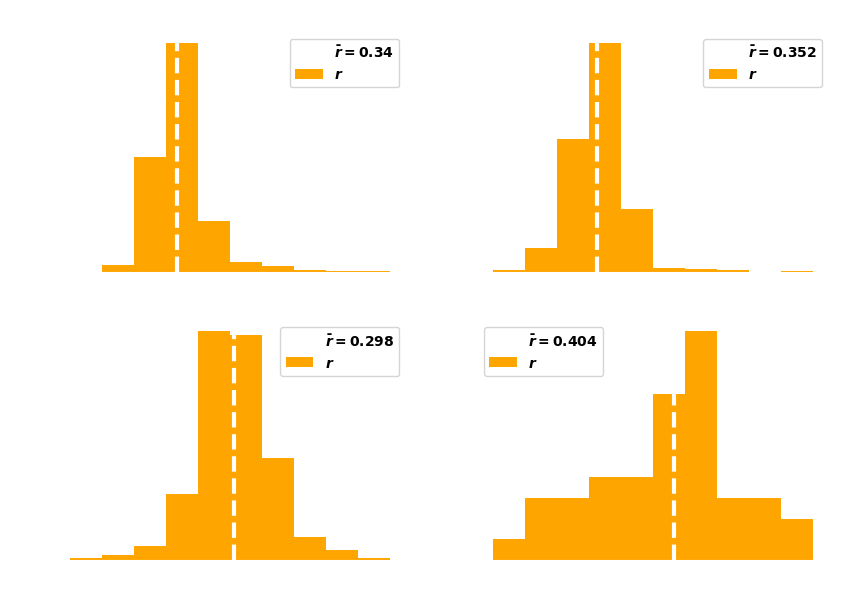
\includegraphics[width=\textwidth]{static/tit_for_tat_r_distributions.png}
        \end{center}
    \end{frame}
    

\begin{frame}
    \begin{center}
    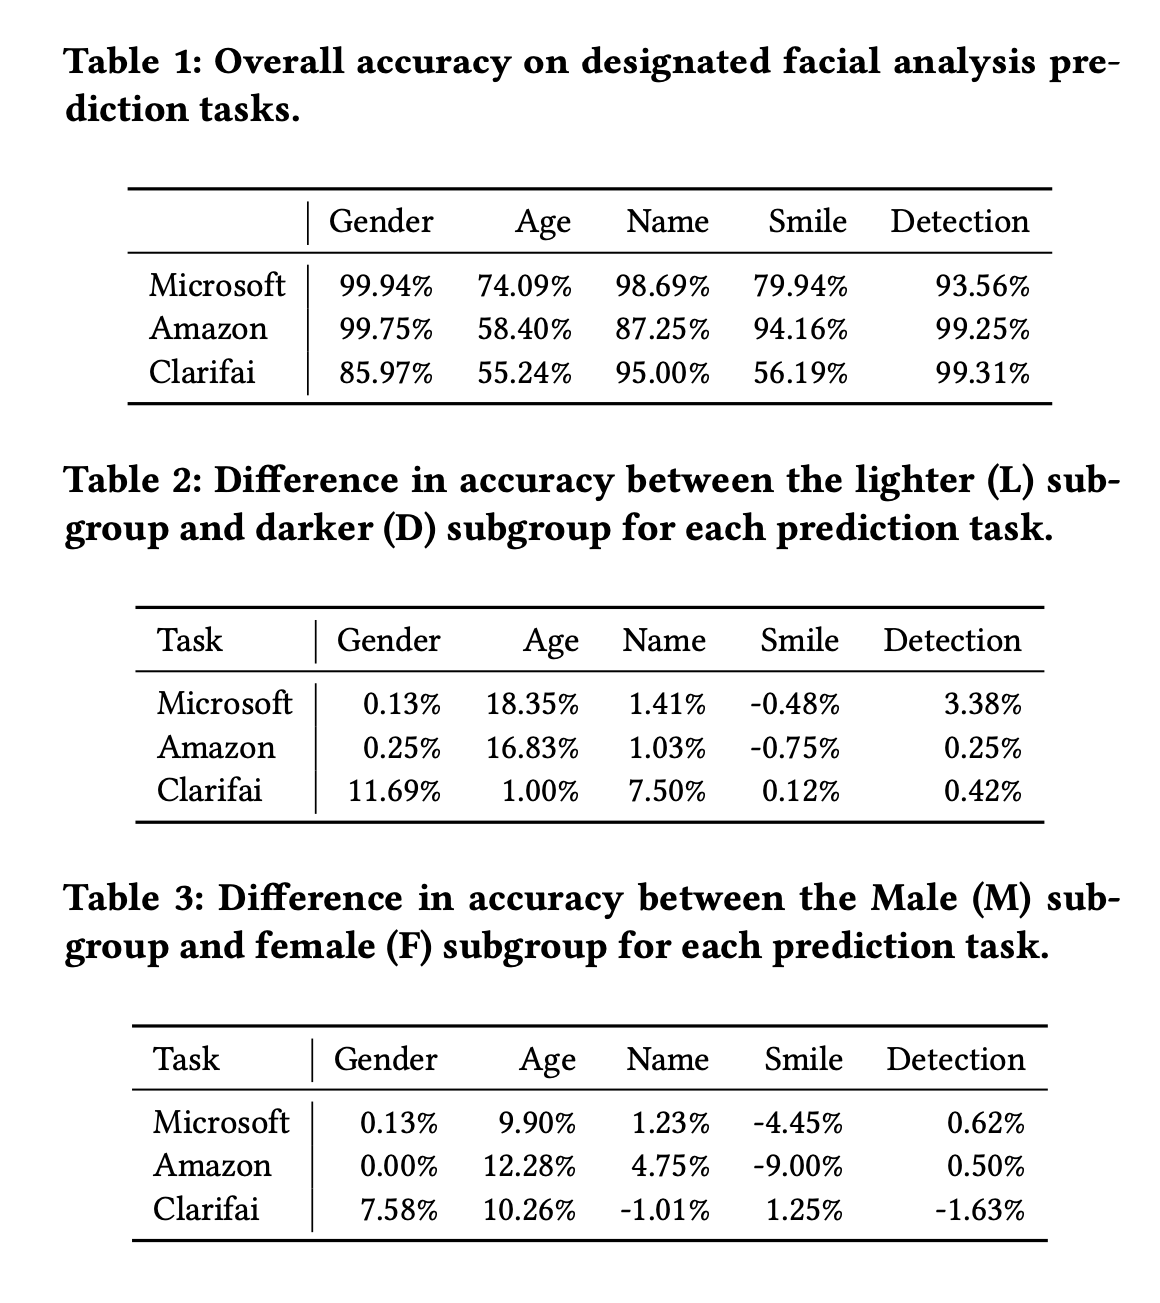
\includegraphics[width=\textwidth]{static/results}
    \end{center}
\end{frame}

\begin{frame}
    \begin{itemize}
    \item \st{Do not be the first to defect} Do not defect on the first turn
    \item \st{Do not be envious} It's okay to be envious 
    \item \st{Do not be too clever} Be clever
    \end{itemize}
\end{frame}

\begin{frame}
    \begin{center}
        Turns + no noise \\
        \vspace{.5cm}

    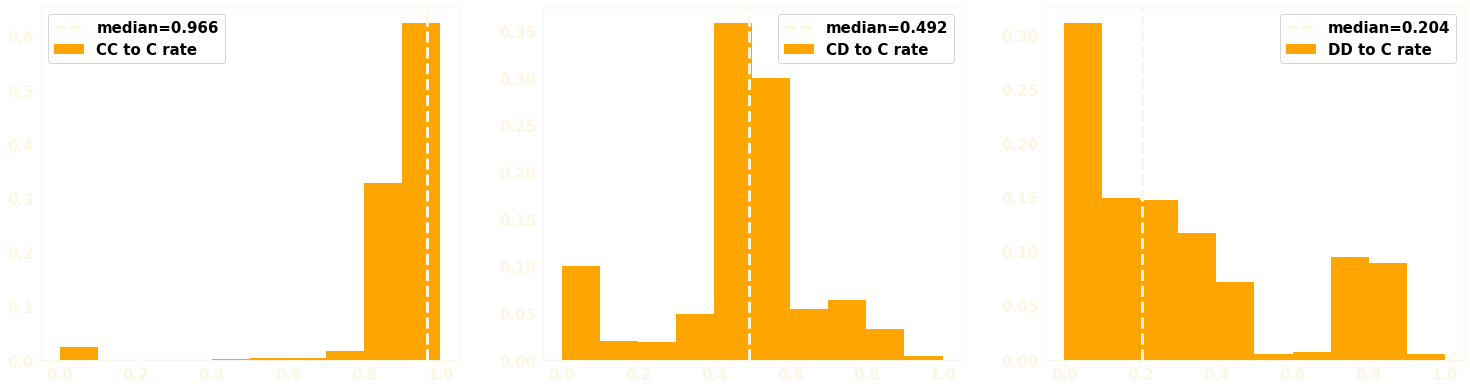
\includegraphics[width=\textwidth]{static/std_states.png}
    \end{center}
\end{frame}

\begin{frame}
    \begin{center}
        Turns + noise \\
        \vspace{.5cm}

    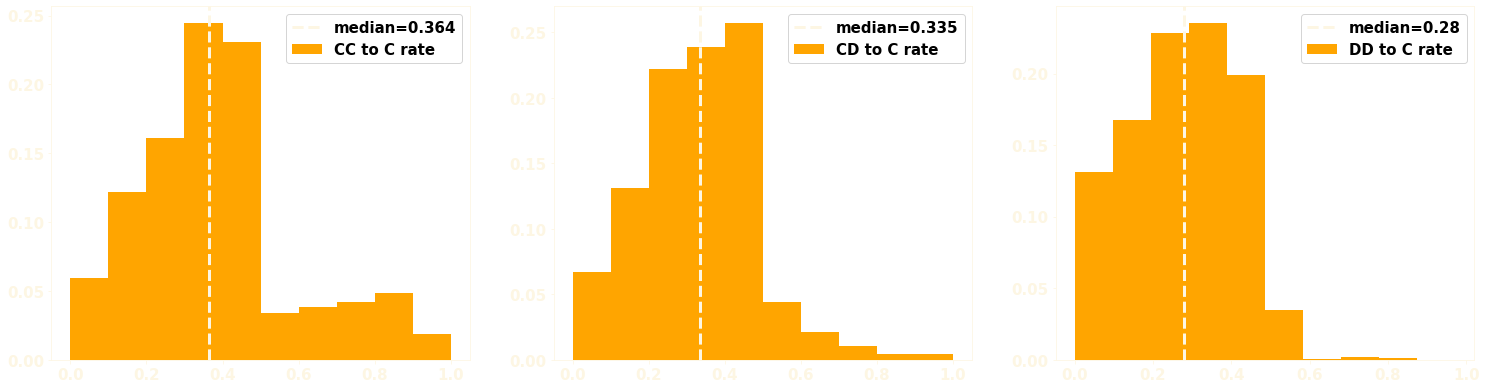
\includegraphics[width=\textwidth]{static/noise_states.png}
    \end{center}
\end{frame}

\begin{frame}
    \begin{center}
        Probabilistic ending + no noise \\
        \vspace{.5cm}

    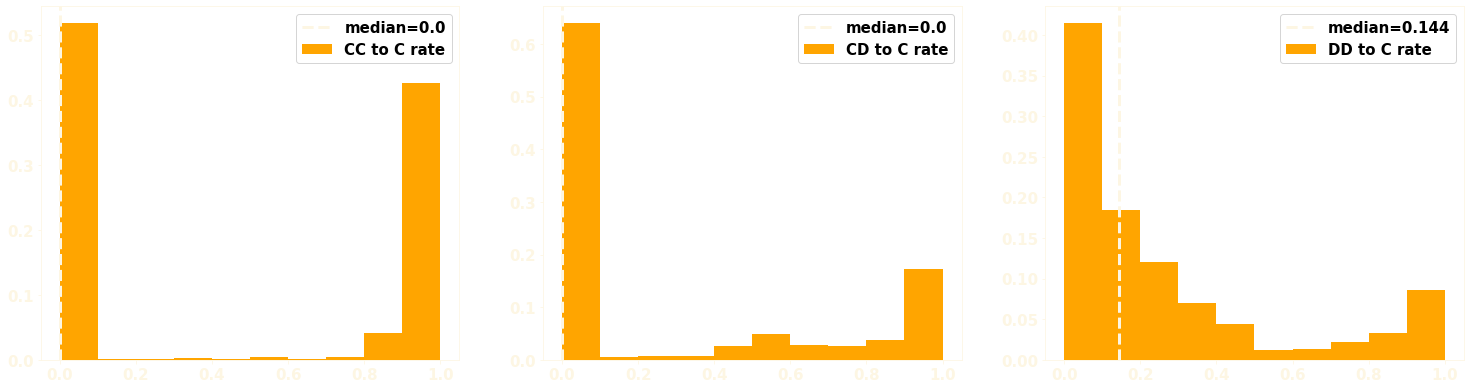
\includegraphics[width=\textwidth]{static/probend_states.png}
    \end{center}
\end{frame}

\begin{frame}
    \begin{itemize}
    \item \st{Do not be the first to defect} Do not defect on the first turn
    \item \st{Do not be envious} It's okay to be envious 
    \item \st{Do not be too clever} Be clever
    \item \st{Be provocable} Be provocable in tournaments with short matches, and generous when matches are longer
    \end{itemize}
\end{frame}

\begin{frame}
    \centering
    Reinforcement Learning Produces Dominant Strategies for the Iterated Prisoner's Dilemma. \\
    \vspace{.5cm}

    \tiny{Marc Harper, Vincent Knight, Martin Jones, Georgios Koutsovoulos, Nikoleta E. Glynatsi, Owen Campbell\\
    \vspace{.5cm}

    doi.org/10.1371/journal.pone.0188046 \\
    \vspace{.5cm}
    
    Axelrod-Python v.2.2.0 - 176 strategies}
\end{frame}

\begin{frame}
    \begin{multicols}{2}
        \begin{itemize}
            \item LookerUp
            \item Gambler
            \item Artificial neural network
            \item Finite state machines
            \item Hidden markov models
            \item Meta strategies
        \end{itemize}
        \end{multicols}
\end{frame}

\begin{frame}
    \begin{center}
    \includestandalone[width=.75\textwidth]{static/lookerup} \\
    \vspace{.5cm}
    \pause

    \small
    \(n_1 = 2, m_1 = 4, m_2 =3 \) \\
    \vspace{.2cm}
    \pause

    EvolvedLookerUp2\_4\_3
    \end{center}
\end{frame}

\begin{frame}
    \begin{center}
        \includestandalone[width=\textwidth]{static/reinforcement}
    \end{center}
\end{frame}

\begin{frame}
    \begin{center}
        \includestandalone[width=.4\textwidth]{static/genetic_algorithm}
    \end{center}
\end{frame}

\begin{frame}
    \begin{center}
    \includestandalone[width=.75\textwidth]{static/gambler}
    \end{center}
\end{frame}

\begin{frame}
    \centering
    \begin{table}
    \resizebox{.55\textwidth}{!}{
\begin{tabular}{lrrrrrrrrr}
    \toprule
    {} &    mean &    std &  min &  max \\
    \midrule
    EvolvedLookerUp2\_2\_2$^{*}$    &   2.173 &  1.070 &    1 &    8 \\
    Evolved HMM 5$^{*}$             &   2.321 &  1.275 &    1 &   10 \\
    Evolved FSM 16$^{*}$            &   2.489 &  1.299 &    1 &   10 \\
    PSO Gambler 2\_2\_2$^{*}$       &   3.961 &  1.525 &    1 &   10 \\
    Evolved FSM 16 Noise 05$^{*}$   &   6.300 &  1.688 &    1 &   11 \\
    PSO Gambler 1\_1\_1$^{*}$       &   7.082 &  2.499 &    1 &   17 \\
    Evolved ANN 5$^{*}$             &   7.287 &  1.523 &    2 &   11 \\
    Evolved FSM 4$^{*}$             &   7.527 &  1.631 &    2 &   12 \\
    Evolved ANN$^{*}$               &   7.901 &  1.450 &    2 &   12 \\
    PSO Gambler Mem1$^{*}$          &   8.222 &  2.535 &    1 &   20 \\
    Evolved ANN 5 Noise 05$^{*}$    &  11.362 &  0.872 &    8 &   16 \\
    DBS                             &  12.197 &  1.125 &    9 &   16 \\
    Winner12                        &  13.221 &  1.137 &    9 &   17 \\
    Fool Me Once                    &  13.960 &  1.083 &    9 &   17 \\
    Omega TFT: 3, 8                 &  14.275 &  1.301 &    9 &   19 \\
    \bottomrule
    \end{tabular}}
    \caption{\tiny{Turns + no noise tournament: Rank in each tournament of top 15 strategies (ranked by median over 50000 tournaments) * indicates that the strategy was trained.}}
    \end{table}
\end{frame}

\begin{frame}
    \centering
    \begin{table}
    \resizebox{.55\textwidth}{!}{
    \begin{tabular}{lrrrrrrrrr}
        \toprule
        {} &    mean &    std &  min  &  max \\
        \midrule
        DBS                                &   1.205 &  0.468 &    1 &    3 \\
        Evolved ANN 5 Noise 05$^{*}$       &   2.184 &  0.629 &    1 &    5 \\
        Evolved FSM 16 Noise 05$^{*}$      &   2.626 &  0.618 &    1 &    9 \\
        Evolved ANN 5$^{*}$                &   6.371 &  2.786 &    2 &   31 \\
        Evolved FSM 4$^{*}$                &   7.919 &  3.175 &    3 &   33 \\
        Evolved HMM 5$^{*}$                &   7.996 &  3.110 &    3 &   26 \\
        Level Punisher                     &   8.337 &  3.083 &    3 &   26 \\
        Omega TFT: 3, 8                    &   8.510 &  3.249 &    3 &   32 \\
        Spiteful Tit For Tat               &   9.159 &  3.772 &    3 &   40 \\
        Evolved FSM 16$^{*}$               &  10.218 &  4.099 &    3 &   56 \\
        PSO Gambler 2\_2\_2 Noise 05$^{*}$ &  10.760 &  4.102 &    3 &   47 \\
        Evolved ANN$^{*}$                  &  11.346 &  3.252 &    3 &   32 \\
        Adaptive                           &  11.420 &  5.739 &    3 &   63 \\
        Math Constant Hunter               &  14.668 &  3.788 &    3 &   43 \\
        Gradual                            &  15.163 &  3.672 &    4 &   49 \\
        \bottomrule
    \end{tabular}}
    \caption{\tiny{Turns + noise tournament: Rank in each tournament of top 15 strategies (ranked by median over 50000 tournaments) * indicates that the strategy was trained.}}
\end{table}
\end{frame}

\begin{frame}
    \begin{center}
    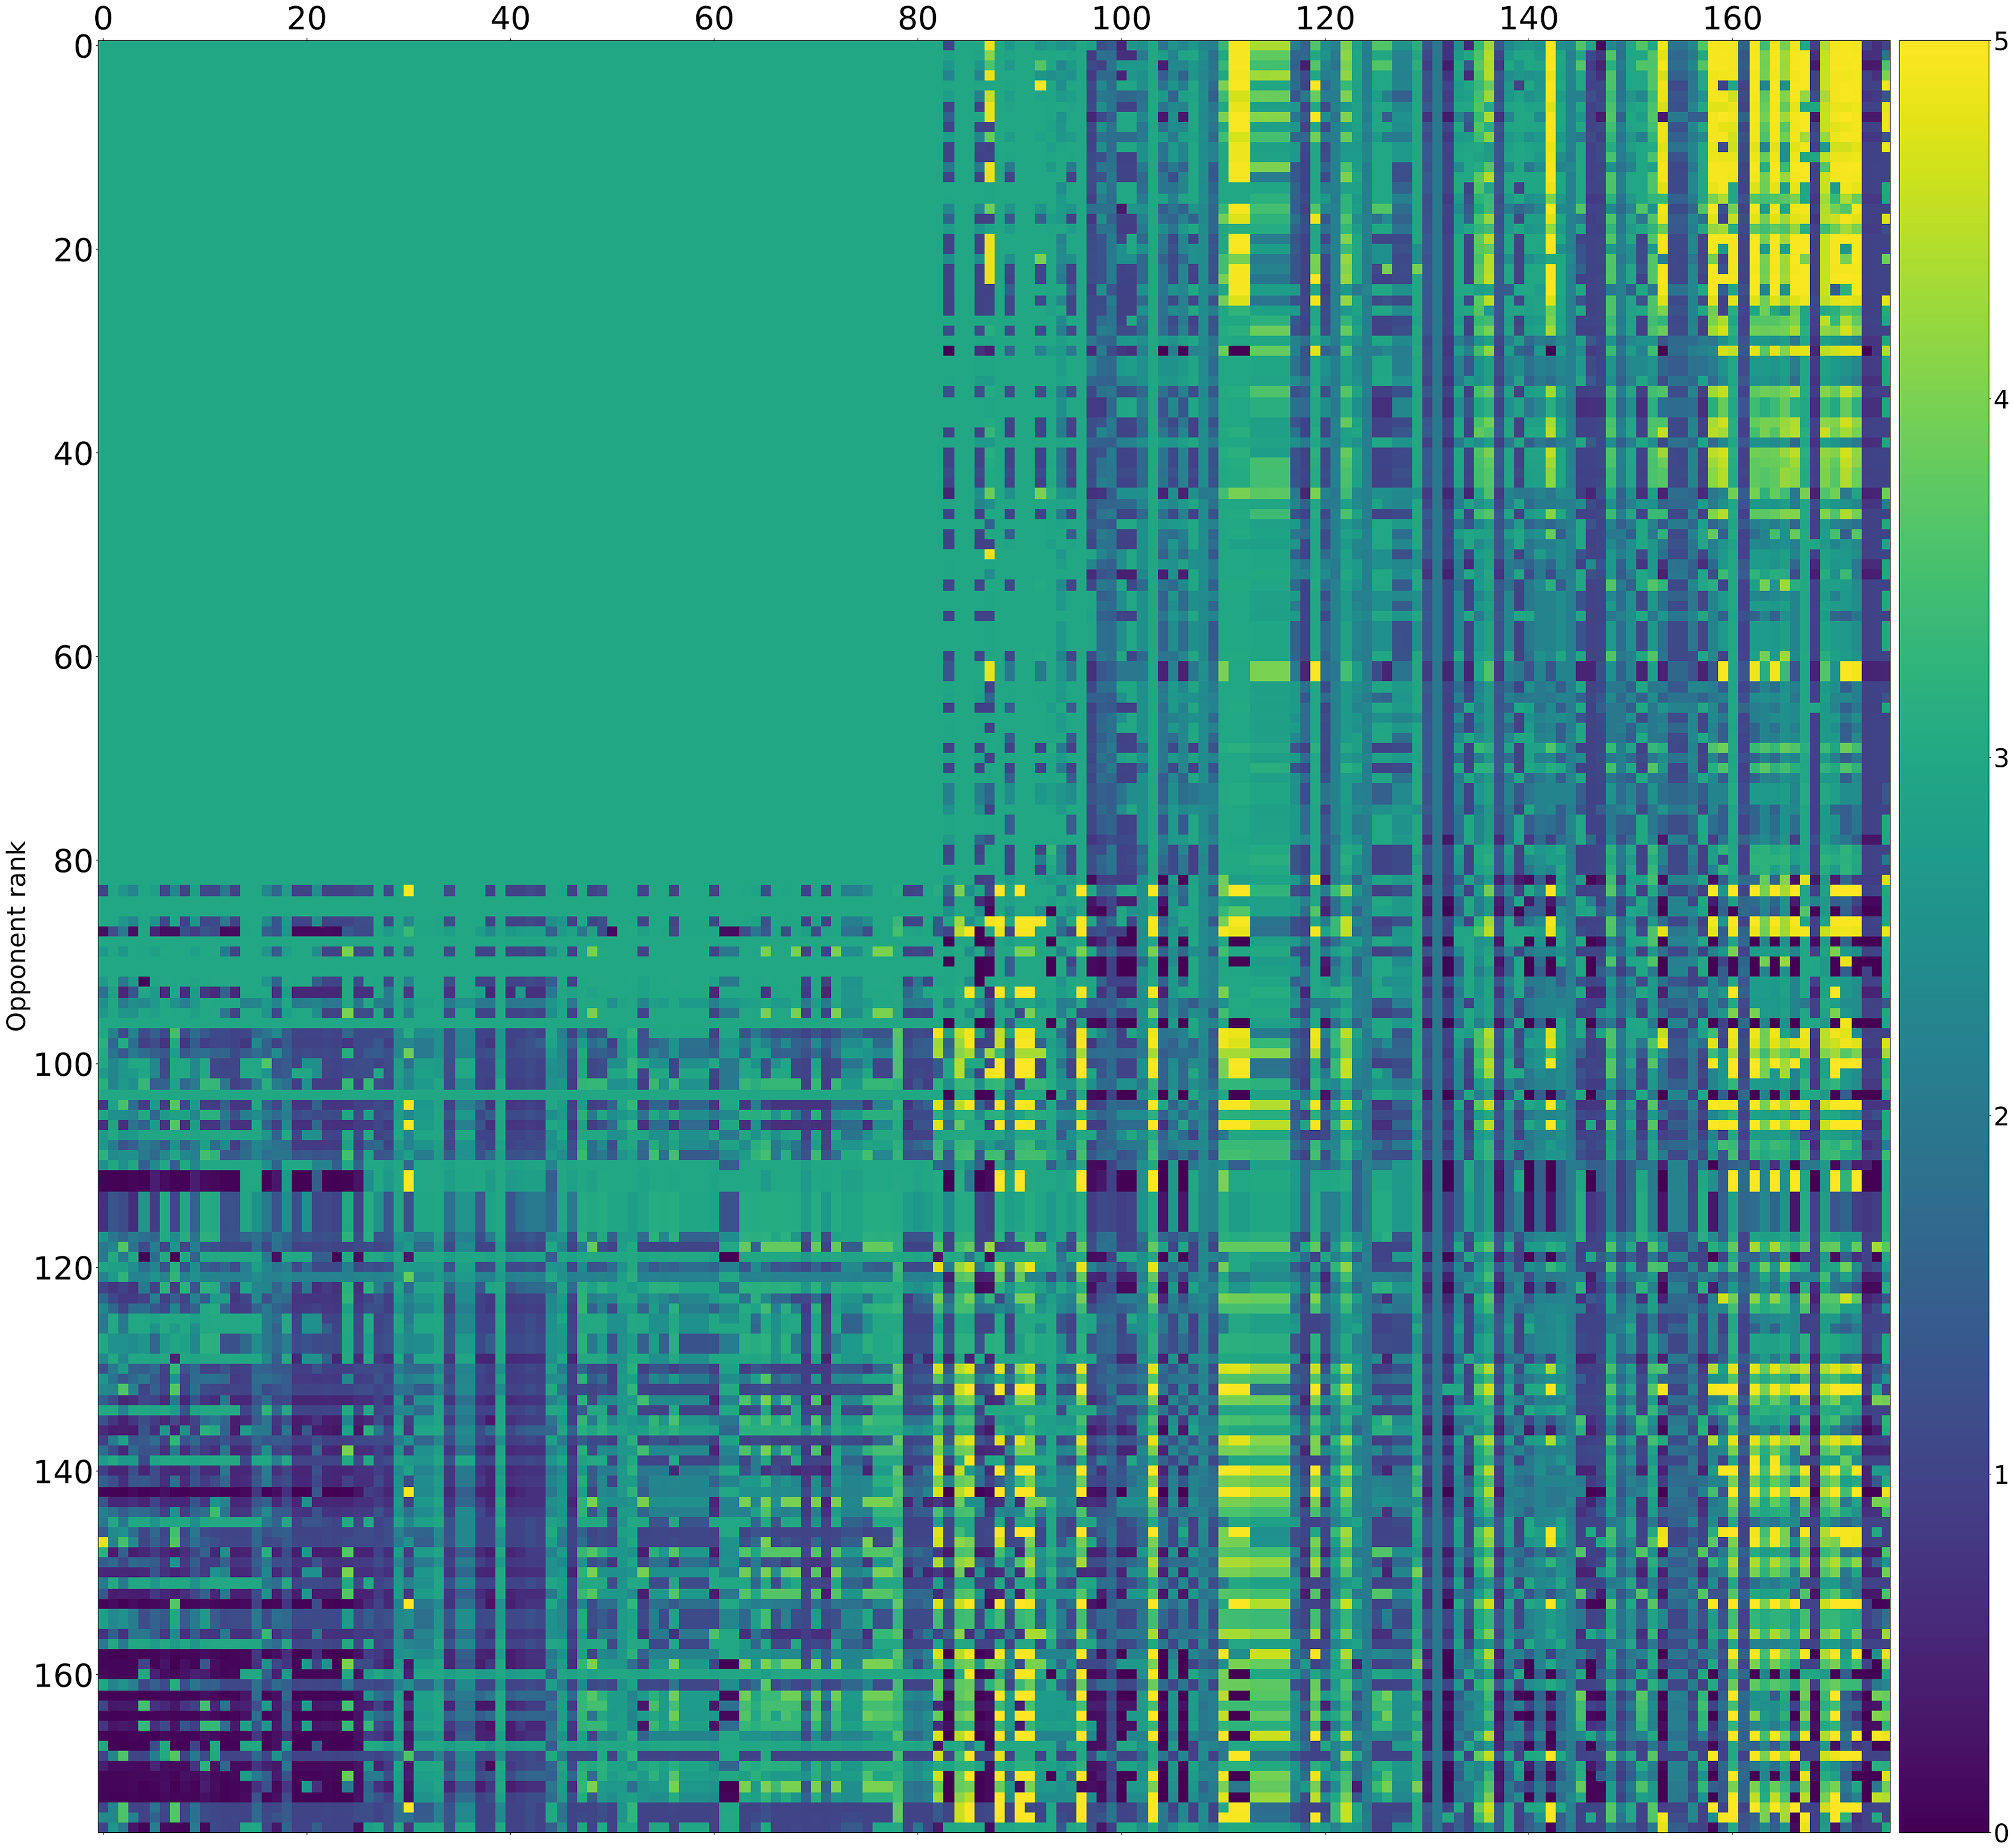
\includegraphics[width=.75\textwidth]{static/interactions.png}
    \end{center}
\end{frame}

\begin{frame}
    \centering
    Evolution Reinforces Cooperation with the Emergence of Self-Recognition Mechanisms: an empirical study of the Moran process for the iterated Prisoner's dilemma \\
    \vspace{.5cm}
    \tiny{
    Vincent Knight, Marc Harper, Nikoleta E. Glynatsi, Owen Campbell \\
    \vspace{.5cm}

    doi.org/10.1371/journal.pone.0204981}
\end{frame}

% \begin{frame}
%     \begin{center}
%     \includestandalone[width=\textwidth]{static/evolutionary_training}
%     \end{center}
% \end{frame}

\begin{frame}
    \begin{center}
    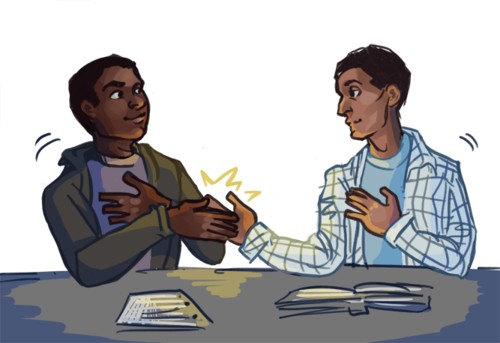
\includegraphics[width=.75\textwidth]{static/handshake.png}
    \end{center}
\end{frame}

\begin{frame}
    \begin{columns}
        \begin{column}{.6\textwidth}
            \begin{center}
                \scalebox{.49}{
                    \documentclass{standalone}

\usepackage{tikz}
\usepackage{standalone}
\usetikzlibrary{calc}

\begin{document}
    \begin{tikzpicture}

    \tikzstyle{state}=[minimum width=0.8cm, font=\boldmath];
    \node[circle, draw=solarizedBase3, thick] (5) at (0, 0) [state] {$6$};
	\node[circle, draw=solarizedBase3, thick] (2) at (4, 0) [state] {$3$};
	\node[circle, draw=solarizedBase3, thick] (15) at (-2, -2) [state] {$16$};
	\node[circle, draw=solarizedBase3, thick] (8) at ($(2)+(2,-2)$) [state] {$9$};
	\node[circle, draw=solarizedBase3, thick] (10) at ($(15)+(4, 0)$) [state] {$11$};
	
	\node[circle, draw=solarizedBase3, thick] (7) at ($(5)+(-1,-4)$) [state] {$8$};
	\node[circle, draw=solarizedBase3, thick] (11) at ($(7)+(2, 0)$) [state] {$12$};



	\node[circle, draw=solarizedBase3, thick] (9) at ($(10)+(0,-4)$) [state] {$10$};
	\node[circle, draw=solarizedBase3, thick] (0) at ($(9)+(-5,0)$) [state] {$1$};
	\node[circle, draw=solarizedBase3, thick] (14) at ($(9)+(5,0)$) [state] {$15$};

	\node[circle, draw=solarizedBase3, thick] (1) at ($(0)+(0,-2)$) [state] {$2$};
	\node[circle, draw=solarizedBase3, thick] (4) at ($(1)+(2,0)$) [state] {$5$};
	\node[circle, draw=solarizedBase3, thick] (6) at ($(4)+(4,0)$) [state] {$7$};
	\node[circle, draw=solarizedBase3, thick] (13) at ($(6)+(2,0)$) [state] {$14$};

	\node[circle, draw=solarizedBase3, thick] (3) at ($(4)+(0,-2)$) [state] {$4$};
	\node[circle, draw=solarizedBase3, thick] (12) at ($(6)+(0,-2)$) [state] {$13$};


    \coordinate[left of=0] (s);

    \draw (s) edge[out=0, in=180, ->, thick] node [above] {$C$} (0);
    \draw (0) edge[out=90, in=135, ->, thick] node [above left] {$C/C$} (7);
    \draw (0) edge[out=-90, in=90, ->, thick] node [left] {$D/C$} (1);

    \draw (1) edge[out=45, in=-135, ->, thick] node [left] {$C/D$} (11);
    \draw (1) edge[out=45, in=-135, ->, thick] node [right] {$D/D$} (11);
    
    \draw (2) edge[out=-45, in=135, ->, thick] node [above right] {$C/D$} (8);
    \draw (2) edge[out=-45, in=135, ->, thick] node [below left] {$D/C$} (8);

    \draw (3) edge[out=180, in=135, ->, thick, loop] node [left] {$C/C$} (3);
    \draw (3) edge[out=0, in=180, ->, thick] node [below] {$D/D$} (12);

    \draw (4) edge[out=0, in=180, ->, thick] node [above] {$C/C$} (6);
    \draw (4) edge[out=-90, in=90, ->, thick] node [left] {$D/C$} (3);

    \draw (5) edge[out=0, in=180, ->, thick] node [below, yshift=-1cm, xshift=2cm] {$D/D$} (8);
    \draw (5) edge[out=-45, in=90, ->, thick] node [left, yshift=-0.8cm, xshift=-0.3cm, rotate=90] {$C/C$} (11);

    \draw (6) edge[out=0, in=180, ->, thick] node [below] {$C/D$} (13);
    \draw (6) edge[out=45, in=180, ->, thick] node [above] {$D/C$} (14);

    \draw (7) edge[out=-135, in=135, ->, thick] node [yshift=1.8cm] {$C/D$} (4);
    \draw (7) edge[out=45, in=180, ->, thick] node [above, yshift=1.2cm, xshift=1.8cm] {$D/D$} (2);

    \draw (8) edge[out=0, in=45, ->, thick, loop] node [above] {$D/D$} (8);
    \draw (8) edge[out=-90, in=130, ->, thick] node [right] {$C/D$} (14);

    \draw (9) edge[out=-135, in=-45, ->, thick] node [above] {$C/C$} (0);
    \draw (9) edge[out=100, in=-100, ->, thick] node [above left, yshift=1.5cm, rotate=90] {$D/D$} (10);

    \draw (10) edge[out=0, in=180, ->, thick] node [below left, xshift=-0.5cm] {$C/C$} (8);
    \draw (10) edge[out=180, in=0, ->, thick] node [above left, xshift=-0.5cm] {$D/C$} (15);

    \draw (11) edge[out=0, in=70, ->, thick] node [above right] {$C/D$} (6);
    \draw (11) edge[out=155, in=-90, ->, thick] node [right, yshift=1cm] {$D/D$} (5);

    \draw (12) edge[out=90, in=-90, ->, thick] node [above right] {$C/D$} (6);
    \draw (12) edge[out=155, in=-90, ->, thick] node [left, yshift=-1cm] {$D/D$} (9);

    \draw (13) edge[out=135, in=0, ->, thick] node [below left, xshift=-0.4cm, yshift=0.4cm] {$C/D$} (9);
    \draw (13) edge[out=70, in=-135, ->, thick] node [right] {$D/D$} (8);

    \draw (14) edge[out=70, in=-45, ->, thick] node [right] {$C/D$} (8);
    \draw (14) edge[out=-90, in=0, ->, thick] node [right] {$D/D$} (13);

    \draw (15) edge[out=-45, in=30, ->, thick] node [left, xshift=-1.8cm, yshift=2.5cm] {$C/C$} (4);
    \draw (15) edge[out=90, in=180, ->, thick] node [above left] {$D/C$} (5);

    \end{tikzpicture}
\end{document}
                }
            \end{center}
        \end{column}
        \begin{column}{.4\textwidth}
            \small
            \begin{tabular}{ll}
                \toprule
                TF1 \#1   & TF1 \#2\\
                \midrule
                \bf{1}: C & \bf{1}: C  \\
                \bf{8}: C & \bf{8}: C  \\
                \bf{5}: D & \bf{5}: D  \\
                4: C      & 4: C  \\
                4: C      & 4: C  \\
                4: C      & 4: C  \\
                4: C      & 4: C  \\
                4: C      & 4: C  \\
                \bottomrule
            \end{tabular}
        \end{column}
    \end{columns}
\end{frame}

\begin{frame}
    \begin{itemize}
    \item \st{Do not be the first to defect} Do not defect on the first turn
    \item \st{Do not be envious} It's okay to be envious 
    \item \st{Do not be too clever} Be clever
    \item \st{Be provocable} Be provocable in tournaments with short matches, and generous when matches are longer
    \item Self recognition mechanism
    \end{itemize}
\end{frame}

\begin{frame}
    \begin{center}
    \faTwitter \ @NikoletaGlyn \\
    \url{http://web.evolbio.mpg.de/social-behaviour/}
    \end{center}
    \vspace{1cm}

    \begin{multicols}{3}
        \begin{itemize}
            \item Vincent Knight
            \item Marc Harper
            \item Owen Campbell
            \item Martin Jones
            \item Georgios Koutsovoulos
        \end{itemize}
        \end{multicols}
\end{frame}

\end{document}